\documentclass{article}
\usepackage{graphicx} 
\usepackage{listings}

\begin{document}

\title{ MapReduce implementation}
\author{Vu Minh Hien Bi12-154}
\date{\today}

\maketitle

\

\maketitle

\section{Code Implementation}

\lstset{language=C++}
\begin{lstlisting}
#include <iostream>
#include <sstream>
#include <map>

void map_function(const std::string& line, std::map<std::string, int>& intermediate_result) {
    std::istringstream iss(line);
    std::string word;
    while (iss >> word) {
        intermediate_result[word]++;
    }
}

void reduce_function(const std::map<std::string, int>& intermediate_result) {
    for (const auto& pair : intermediate_result) {
        std::cout << pair.first << "\t" << pair.second << std::endl;
    }
}

int main() {
    std::map<std::string, int> intermediate_result;

    std::stringstream input_data;
    input_data << "tell me why\n";
    input_data << "ain nothing but heartbreak\n";
    input_data << "tell me why\n";

    std::string line;

    while (std::getline(input_data, line)) {
        map_function(line, intermediate_result);
    }

    reduce_function(intermediate_result);

    return 0;
}
\end{lstlisting}

\section{Explanation}

\subsection{MapReduce Implementation Choice}
\begin{itemize}
    \item \textbf{Simplicity}: The chosen implementation is straightforward and easy to understand, suitable for educational purposes or simple tasks.
    \item \textbf{Familiarity}: This implementation closely resembles the concept of MapReduce, widely used in distributed and parallel computing frameworks for processing large datasets efficiently.
    \item \textbf{C++ Language}: Leveraging standard library features (\texttt{std::map}, \texttt{std::stringstream}, etc.) accomplishes the task without external dependencies.
\end{itemize}

\subsection{Mapper Function}
\begin{itemize}
    \item The \texttt{map\_function} serves as the Mapper. It processes each input line and emits intermediate key-value pairs.
    \item It tokenizes each line into words using \texttt{std::istringstream}, then updates a map (\texttt{intermediate\_result}) with the count of each word.
    \item For each word encountered, it increments the count in the map.
\end{itemize}

\subsection{Reducer Function}
\begin{itemize}
    \item The \texttt{reduce\_function} serves as the Reducer. It aggregates intermediate results produced by the Mapper.
    \item It takes the intermediate result (the map containing word counts) as input and prints out each word along with its count.
    \item In this case, the Reducer function does not perform aggregation since it's a single-machine implementation. In a distributed setting, the Reducer would combine counts for the same word emitted by different mappers.
\end{itemize}

\subsection{Who Does What}
\begin{itemize}
    \item \textbf{Mapper}: Processes data and emits intermediate results.
    \item \textbf{Reducer}: Aggregates intermediate results to produce the final output.
    \item \textbf{Main Function}: Orchestrates execution by feeding input data, invoking the Mapper for each input line, and calling the Reducer to output the final result.
\end{itemize}

\section{Result}

\begin{figure}[h]
    \centering
    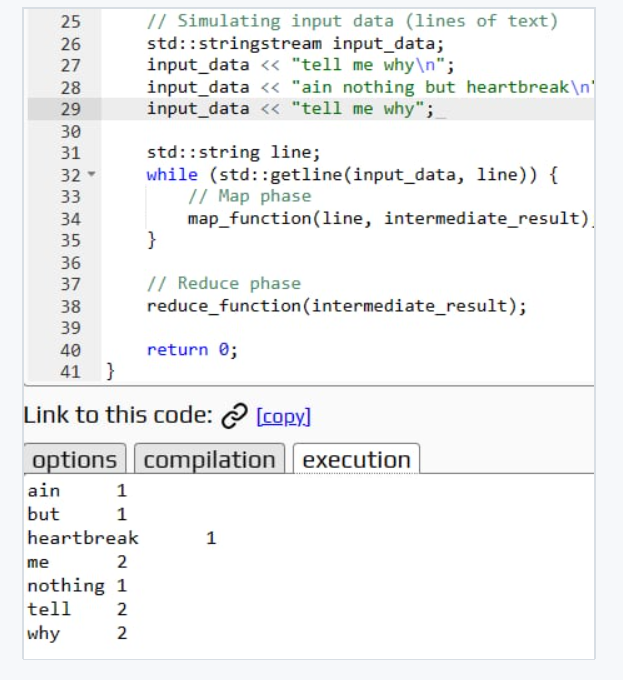
\includegraphics[width=0.8\textwidth]{wordcount.png} 
    \caption{Result}
    \label{fig:output}
\end{figure}




\end{document}

